% !TEX spellcheck = en_US



% ~~~~~~~~~~~~~~~~~~~~~~~~~~~~~~~~~~~~~~~ V
% (NC) 2026 Haluk Bingol
% github.com/halukbingol/LaTeX-Templates
%
% Licensees may copy, distribute, display, and perform the work and make derivative works 
% and remixes based on it only for non-commercial purposes. 
% ~~~~~~~~~~~~~~~~~~~~~~~~~~~~~~~~~~~~~~~ A




% v20261030T1200

\documentclass[aspectratio=169,10pt,compress]{beamer}




% ~~~~~~~~~~~~~~~~~~~~~~~~~~~~~~~~~~~~~~~~~~~~~~~~~~~~~~~~~~~~~~~~~ V hblib
	\usepackage{../../hblib/hblibPresentation} % lib presentation: theme, i/N, \hSection, algorithm2e, ...
	\usepackage{../../hblib/hblibCodeoutput} % lib code + output: \lstcode, \lstterminal, ...
	\usepackage{../../hblib/hblibDatastructures} % lib data structures: \hString, \hStack, \hQueue, \hArray, \hGrid
% ~~~~~~~~~~~~~~~~~~~~~~~~~~~~~~~~~~~~~~~~~~~~~~~~~~~~~~~~~~~~~~~~~ A hblib




% +++++++++++++++++++++++++++++++++++++++ V specific
\DontPrintSemicolon % in algorithms
\SetKw{KwAnd}{and}
\SetKw{KwNot}{not}
% +++++++++++++++++++++++++++++++++++++++ A specific



\title[Arrays ND: Concepts]{
	Multi-Dimensional Arrays\\
	Concepts
}
\subtitle{
	\cisOOO\ -- Level 0: ideas and pictures
}
\author[Erkovan]{Sait Erkovan}

\institute[FCIS]{
	Faculty of Computer and Information Sciences\\
	Yeditepe University
}
\date{{\tiny \hbTimeStamp}}

\begin{document}




% ~~~~~~~~~~~~~~~~~~~~~~~~~~~~~~~~~~~~~~ V frm
\begin{frame}[t,fragile]
	\titlepage
\end{frame}
% ~~~~~~~~~~~~~~~~~~~~~~~~~~~~~~~~~~~~~~ A frm




% ~~~~~~~~~~~~~~~~~~~~~~~~~~~~~~~~~~~~~~ V frm
\begin{frame}[t,fragile] \frametitle{Outline}
	\begin{columns}[T]
		\begin{column}{0.48\textwidth}
			\tableofcontents[sections={1-4}, hideallsubsections]
		\end{column}
		\begin{column}{0.48\textwidth}
			\tableofcontents[sections={5-7}, hideallsubsections]
		\end{column}
	\end{columns}

	\vspace{1em}
	\small This deck has ideas, pictures and pseudo code only; it builds on \hCode{array1D-0-concepts}.
	The same ideas as Java programs: \hCode{arrayND-5-examples}.
\end{frame}
% ~~~~~~~~~~~~~~~~~~~~~~~~~~~~~~~~~~~~~~ A frm




% ~~~~~~~~~~~~~~~~~~~~~~~~~~~~~~~~~~~~~~ V
\hSection[Why]{Why tables?}
% ~~~~~~~~~~~~~~~~~~~~~~~~~~~~~~~~~~~~~~ A




% ~~~~~~~~~~~~~~~~~~~~~~~~~~~~~~~~~~~~~~ V frm
\begin{frame}[t,fragile] \frametitle{From lists to a table}
	\begin{columns}[T]
		\begin{column}{0.44\textwidth}
			\textbf{Three lists}

			\vspace{0.6em}
			\begin{tikzpicture}
				\hArray[id=a, name={ali}, width=0.6, index=none]{72,85,90,64}
				\hArray[id=b, at={(0,-0.8)}, name={bora}, width=0.6, index=none]{55,61,70,80}
				\hArray[id=c, at={(0,-1.6)}, name={can}, width=0.6, index=none]{90,88,93,99}
			\end{tikzpicture}
		\end{column}
		\begin{column}{0.52\textwidth}
			\textbf{One table}

			\vspace{0.6em}
			\begin{tikzpicture}
				\hGrid[id=s, name={scores}, width=0.6]{{72,85,90,64},{55,61,70,80},{90,88,93,99}}
			\end{tikzpicture}
		\end{column}
	\end{columns}

	\vspace{1em}
	\begin{itemize}
		\item A \hDefined{table} (a two-dimensional array) holds values of one type in \hDefined{rows} and \hDefined{columns}
		\item One name, two numbers: the row and the column choose a \hDefined{cell}
		\item Lists of the same length that belong together are the rows of one table
	\end{itemize}
\end{frame}
% ~~~~~~~~~~~~~~~~~~~~~~~~~~~~~~~~~~~~~~ A frm




% ~~~~~~~~~~~~~~~~~~~~~~~~~~~~~~~~~~~~~~ V frm
\begin{frame}[t,fragile] \frametitle{Questions about a table}


% +++++++++++++++++++++++++++++++++++++++ V tbl
%: -Tbl. questions
\begin{table}
		\small
		\begin{tabular}{@{}L{0.42\textwidth}L{0.22\textwidth}L{0.28\textwidth}@{}}
			\toprule
			\textbf{Question} & \textbf{What is visited} & \textbf{Answer} \\
			\midrule
			How did student 1 do in quiz 2?          & one cell        & one number \\
			What is the total of each student?       & every row       & one number per row \\
			What is the average of each quiz?        & every column    & one number per column \\
			What is the best score of the class?     & every cell      & a value and its place \\
			Who scored 90 or more in quiz 3?         & one column      & a list of rows \\
			\bottomrule
		\end{tabular}
\end{table}%
% +++++++++++++++++++++++++++++++++++++++ A tbl


	\vspace{0.5em}
	\small Before writing a loop, ask: one cell, one row, one column, or the whole table?
\end{frame}
% ~~~~~~~~~~~~~~~~~~~~~~~~~~~~~~~~~~~~~~ A frm




% ~~~~~~~~~~~~~~~~~~~~~~~~~~~~~~~~~~~~~~ V
\hSection[Anatomy]{Anatomy of a table}
% ~~~~~~~~~~~~~~~~~~~~~~~~~~~~~~~~~~~~~~ A




% ~~~~~~~~~~~~~~~~~~~~~~~~~~~~~~~~~~~~~~ V frm
\begin{frame}[t,fragile] \frametitle{Rows, columns, cells}
	\begin{center}
		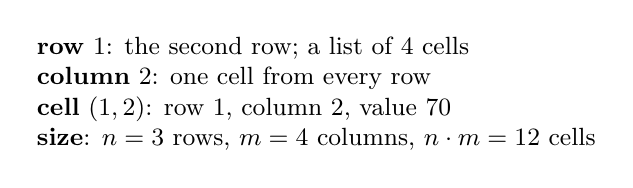
\begin{tikzpicture}
			\hGrid[id=g, name={t}, width=0.8, rowhot={1}, colhot={2}, hot={1/2}]{{72,85,90,64},{55,61,70,80},{90,88,93,99}}
			\node[font=\small, anchor=west, align=left] at (4.0,-0.25) {%
				\textbf{row} 1: the second row; a list of 4 cells\\
				\textbf{column} 2: one cell from every row\\
				\textbf{cell} $(1, 2)$: row 1, column 2, value 70\\
				\textbf{size}: $n = 3$ rows, $m = 4$ columns, $n \cdot m = 12$ cells};
		\end{tikzpicture}
	\end{center}

	\begin{itemize}\small
		\item Both indices start at 0, as in a list: rows $0 \dots n - 1$, columns $0 \dots m - 1$
		\item Every row of this table has the same length: it is \hDefined{rectangular}
		\item All cells have one type; the sizes are fixed when the table is made (the rules of a list)
	\end{itemize}
\end{frame}
% ~~~~~~~~~~~~~~~~~~~~~~~~~~~~~~~~~~~~~~ A frm




% ~~~~~~~~~~~~~~~~~~~~~~~~~~~~~~~~~~~~~~ V frm
\begin{frame}[t,fragile] \frametitle{Row first, then column}
	\begin{columns}[T]
		\begin{column}{0.46\textwidth}
			\begin{center}
				\begin{tikzpicture}
					\hGrid[id=m, width=0.55, hot={1/4}]{{.,.,.,.,.,.},{.,.,.,.,*,.},{.,.,.,.,.,.}}
					\draw[->, thick, colorIndex] (-0.6,0.5) -- (-0.6,-1.0) node[midway, left, font=\scriptsize] {$r$, $y$};
					\draw[->, thick, colorIndex] (0,0.95) -- (3.3,0.95) node[midway, above, font=\scriptsize] {$c$, $x$};
				\end{tikzpicture}
			\end{center}
		\end{column}
		\begin{column}{0.50\textwidth}
			\begin{itemize}\small
				\item The first index picks the row: it goes \emph{down}
				\item The second index picks the column: it goes \emph{right}
				\item A point $(x, y) = (4, 1)$ of a picture is the cell $(1, 4)$: row $y$, column $x$
			\end{itemize}
		\end{column}
	\end{columns}

	\vspace{1em}
	\small \hRemark{A common slip}: writing $(x, y)$ in the order of mathematics gives (column, row). Name the indices
	\emph{row} and \emph{column}, or $r$ and $c$, and keep this order everywhere.
\end{frame}
% ~~~~~~~~~~~~~~~~~~~~~~~~~~~~~~~~~~~~~~ A frm




% ~~~~~~~~~~~~~~~~~~~~~~~~~~~~~~~~~~~~~~ V frm
\begin{frame}[t,fragile] \frametitle{Row-major order: numbering the cells}
	\begin{columns}[T]
		\begin{column}{0.40\textwidth}
			\begin{center}
				\begin{tikzpicture}
					\hGrid[id=k, width=0.7, hot={2/1}]{{0,1,2,3},{4,5,6,7},{8,9,10,11}}
				\end{tikzpicture}
			\end{center}
		\end{column}
		\begin{column}{0.56\textwidth}
			Visit the rows one after the other and count the cells: \hDefined{row-major order}.
			For a table with $m$ columns:
			\[
				k = r \cdot m + c, \qquad r = \lfloor k / m \rfloor, \qquad c = k \bmod m
			\]
			Cell $(2, 1)$ is number $2 \cdot 4 + 1 = 9$.
		\end{column}
	\end{columns}

	\vspace{0.8em}
	\begin{itemize}\small
		\item The same table fits in one list of $n \cdot m$ values: cell $(r, c)$ goes to position $k$
		\item Reading a table row by row follows this numbering; column by column jumps $m$ places at a time
	\end{itemize}
\end{frame}
% ~~~~~~~~~~~~~~~~~~~~~~~~~~~~~~~~~~~~~~ A frm




% ~~~~~~~~~~~~~~~~~~~~~~~~~~~~~~~~~~~~~~ V
\hSection[Rows]{A table is an array of rows}
% ~~~~~~~~~~~~~~~~~~~~~~~~~~~~~~~~~~~~~~ A




% ~~~~~~~~~~~~~~~~~~~~~~~~~~~~~~~~~~~~~~ V frm
\begin{frame}[t,fragile] \frametitle{Rows are lists}
	\begin{center}
		\begin{tikzpicture}
			\node[hvar] (v) at (0,0.25) {};
			\node[font=\ttfamily\small, left=2pt of v] {t};
			\hArray[id=o, at={(1.2,-0.35)}, width=0.6, index=none]{\phantom{0},\phantom{0},\phantom{0}}
			\hArray[id=a, at={(4.0,1.0)}, width=0.6]{72,85,90,64}
			\hArray[id=b, at={(4.0,0.0)}, width=0.6]{55,61,70,80}
			\hArray[id=c, at={(4.0,-1.0)}, width=0.6]{90,88,93,99}
			\draw[href] (v.center) -- (o-0.west);
			\draw[href] (o-0.center) -- (a-0.west);
			\draw[href] (o-1.center) -- (b-0.west);
			\draw[href] (o-2.center) -- (c-0.west);
			\node[font=\small, anchor=west] at (6.6,1.25) {row 0};
			\node[font=\small, anchor=west] at (6.6,0.25) {row 1};
			\node[font=\small, anchor=west] at (6.6,-0.75) {row 2};
		\end{tikzpicture}
	\end{center}

	\begin{itemize}
		\item In Java a table is a list whose elements are \emph{references to rows}; every row is an ordinary list
		\item Row $r$ is a whole list: everything of \hCode{array1D} (length, loops, patterns) works on it
		\item Two references to the same row make the row shared: a change through one is seen through the other
	\end{itemize}
\end{frame}
% ~~~~~~~~~~~~~~~~~~~~~~~~~~~~~~~~~~~~~~ A frm




% ~~~~~~~~~~~~~~~~~~~~~~~~~~~~~~~~~~~~~~ V frm
\begin{frame}[t,fragile] \frametitle{Rectangular or ragged}
	\begin{columns}[T]
		\begin{column}{0.48\textwidth}
			\textbf{Rectangular}: every row has $m$ cells

			\vspace{0.8em}
			\begin{tikzpicture}
				\hGrid[id=r, width=0.6, index=rows]{{0,0,0,0},{0,0,0,0},{0,0,0,0}}
			\end{tikzpicture}
		\end{column}
		\begin{column}{0.48\textwidth}
			\textbf{Ragged}: each row has its own length

			\vspace{0.8em}
			\begin{tikzpicture}
				\hGrid[id=j, width=0.6, index=rows]{{1},{1,1},{1,2,1},{1,3,3,1}}
			\end{tikzpicture}
		\end{column}
	\end{columns}

	\vspace{0.8em}
	\begin{itemize}\small
		\item Because rows are separate lists, they need not be equal: a \hDefined{ragged} (jagged) table
		\item Use it when rows really differ: a triangle, a month per row, seats per row of a theater
		\item ``The number of columns'' then has no meaning: ask for the length of row $r$
	\end{itemize}
\end{frame}
% ~~~~~~~~~~~~~~~~~~~~~~~~~~~~~~~~~~~~~~ A frm




% ~~~~~~~~~~~~~~~~~~~~~~~~~~~~~~~~~~~~~~ V frm
\begin{frame}[t,fragile] \frametitle{Copying a table: references or cells?}
	\begin{center}
		\begin{tikzpicture}
			\node[font=\small] at (1.0,1.55) {\textbf{shallow copy}};
			\hArray[id=o, at={(0,0)}, width=0.5, index=none, name={a}]{\phantom{0},\phantom{0}}
			\hArray[id=p, at={(0,-1.0)}, width=0.5, index=none, name={b}]{\phantom{0},\phantom{0}}
			\hArray[id=r0, at={(2.2,0.6)}, width=0.5, index=none]{1,2}
			\hArray[id=r1, at={(2.2,-0.6)}, width=0.5, index=none]{3,4}
			\draw[href] (o-0.center) -- (r0-0.west);
			\draw[href] (o-1.center) -- (r1-0.west);
			\draw[href] (p-0.center) -- (r0-0.south west);
			\draw[href] (p-1.center) -- (r1-0.south west);

			\node[font=\small] at (7.0,1.55) {\textbf{deep copy}};
			\hArray[id=q, at={(6.0,0)}, width=0.5, index=none, name={a}]{\phantom{0},\phantom{0}}
			\hArray[id=w, at={(6.0,-1.0)}, width=0.5, index=none, name={c}]{\phantom{0},\phantom{0}}
			\hArray[id=s0, at={(8.0,0.8)}, width=0.5, index=none]{1,2}
			\hArray[id=s1, at={(8.0,0.0)}, width=0.5, index=none]{3,4}
			\hArray[id=u0, at={(8.0,-0.8)}, width=0.5, index=none]{1,2}
			\hArray[id=u1, at={(8.0,-1.6)}, width=0.5, index=none]{3,4}
			\draw[href] (q-0.center) -- (s0-0.west);
			\draw[href] (q-1.center) -- (s1-0.west);
			\draw[href] (w-0.center) -- (u0-0.west);
			\draw[href] (w-1.center) -- (u1-0.west);
		\end{tikzpicture}
	\end{center}

	\begin{itemize}\small
		\item \hDefined{Shallow}: copy only the list of references; both tables share the rows
		\item \hDefined{Deep}: copy every row too; the two tables have nothing in common
		\item With rows shared, changing \hCode{b}'s cell $(0, 0)$ changes \hCode{a}'s cell $(0, 0)$
	\end{itemize}
\end{frame}
% ~~~~~~~~~~~~~~~~~~~~~~~~~~~~~~~~~~~~~~ A frm




% ~~~~~~~~~~~~~~~~~~~~~~~~~~~~~~~~~~~~~~ V
\hSection[Visits]{Visiting the cells}
% ~~~~~~~~~~~~~~~~~~~~~~~~~~~~~~~~~~~~~~ A




% ~~~~~~~~~~~~~~~~~~~~~~~~~~~~~~~~~~~~~~ V frm
\begin{frame}[t,fragile] \frametitle{Row by row}
	\begin{columns}[T]
		\begin{column}{0.44\textwidth}


% +++++++++++++++++++++++++++++++++++++++ V alg
%: -Alg. row by row
\begin{algorithm}[H]
				\caption{RowByRow($t$)}
				\For{$r \gets 0$ \KwTo $n - 1$}{
				    \For{$c \gets 0$ \KwTo (length of row $r$) $- 1$}{
				        visit $t[r][c]$\;
				    }
				}
\end{algorithm}
% +++++++++++++++++++++++++++++++++++++++ A alg

		\end{column}
		\begin{column}{0.52\textwidth}
			\begin{center}
				\begin{tikzpicture}
					\hGrid[id=o, width=0.6]{{1,2,3,4},{5,6,7,8},{9,10,11,12}}
				\end{tikzpicture}
			\end{center}
			\small The numbers show the order of the visits.
		\end{column}
	\end{columns}

	\vspace{0.5em}
	\begin{itemize}\small
		\item The outer loop picks a row, the inner loop walks along it: two nested loops
		\item The inner bound is the length of \emph{this} row, so ragged tables work too
		\item This order is row-major order: the natural order for a table stored as rows
	\end{itemize}
\end{frame}
% ~~~~~~~~~~~~~~~~~~~~~~~~~~~~~~~~~~~~~~ A frm




% ~~~~~~~~~~~~~~~~~~~~~~~~~~~~~~~~~~~~~~ V frm
\begin{frame}[t,fragile] \frametitle{Column by column}
	\begin{columns}[T]
		\begin{column}{0.44\textwidth}


% +++++++++++++++++++++++++++++++++++++++ V alg
%: -Alg. column by column
\begin{algorithm}[H]
				\caption{ColumnByColumn($t$), rectangular}
				\For{$c \gets 0$ \KwTo $m - 1$}{
				    \For{$r \gets 0$ \KwTo $n - 1$}{
				        visit $t[r][c]$\;
				    }
				}
\end{algorithm}
% +++++++++++++++++++++++++++++++++++++++ A alg

		\end{column}
		\begin{column}{0.52\textwidth}
			\begin{center}
				\begin{tikzpicture}
					\hGrid[id=o, width=0.6]{{1,4,7,10},{2,5,8,11},{3,6,9,12}}
				\end{tikzpicture}
			\end{center}
			\small The loops are swapped; the cell is still $t[r][c]$.
		\end{column}
	\end{columns}

	\vspace{0.5em}
	\begin{itemize}\small
		\item Needed for questions about columns: the average of each quiz
		\item Only for rectangular tables: a short row has no cell in a far column
		\item Swap the loops, never the indices: it is still row first, then column
	\end{itemize}
\end{frame}
% ~~~~~~~~~~~~~~~~~~~~~~~~~~~~~~~~~~~~~~ A frm




% ~~~~~~~~~~~~~~~~~~~~~~~~~~~~~~~~~~~~~~ V frm
\begin{frame}[t,fragile] \frametitle{Diagonals of a square table}
	\begin{columns}[T]
		\begin{column}{0.36\textwidth}
			\begin{center}
				\begin{tikzpicture}
					\hGrid[id=d, width=0.6, hot={0/0,1/1,2/2,3/3}, cur={0/3,1/2,2/1,3/0}]{{a,,,b},{,a,b,},{,b,a,},{b,,,a}}
				\end{tikzpicture}
			\end{center}
		\end{column}
		\begin{column}{0.60\textwidth}
			\begin{itemize}\small
				\item In an $n \times n$ table the \hDefined{main diagonal} (a) is the cells $(i, i)$
				\item The other diagonal (b) is $(i, n - 1 - i)$: the column is the mirror of the row
				\item One loop over $i$ visits a diagonal: $n$ cells, not $n^{2}$
				\item Only square tables have both diagonals reaching every row and column
			\end{itemize}
		\end{column}
	\end{columns}
\end{frame}
% ~~~~~~~~~~~~~~~~~~~~~~~~~~~~~~~~~~~~~~ A frm




% ~~~~~~~~~~~~~~~~~~~~~~~~~~~~~~~~~~~~~~ V frm
\begin{frame}[t,fragile] \frametitle{Neighbors and edges}
	\begin{columns}[T]
		\begin{column}{0.38\textwidth}
			\begin{center}
				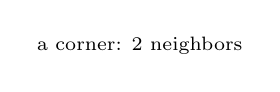
\begin{tikzpicture}
					\hGrid[id=n, width=0.6, index=both, hot={1/2}, cur={0/2,2/2,1/1,1/3}]{{,,,},{,,,},{,,,}}
					\hGrid[id=e, at={(0,-2.3)}, width=0.6, index=none, hot={0/0}, cur={0/1,1/0}]{{,,,},{,,,},{,,,}}
					\node[font=\scriptsize, anchor=north] at (1.2,-3.35) {a corner: 2 neighbors};
				\end{tikzpicture}
			\end{center}
		\end{column}
		\begin{column}{0.58\textwidth}


% +++++++++++++++++++++++++++++++++++++++ V alg
%: -Alg. neighbors
\begin{algorithm}[H]
			\caption{SumOfNeighbors($t, r, c$)}
			$s \gets 0$\;
			\lIf{$r > 0$}{$s \gets s + t[r - 1][c]$}
			\lIf{$r < n - 1$}{$s \gets s + t[r + 1][c]$}
			\lIf{$c > 0$}{$s \gets s + t[r][c - 1]$}
			\lIf{$c < m - 1$}{$s \gets s + t[r][c + 1]$}
			\Return{$s$}\;
\end{algorithm}
% +++++++++++++++++++++++++++++++++++++++ A alg

		\end{column}
	\end{columns}

	\vspace{0.3em}
	\begin{itemize}\small
		\item Inside, a cell has 4 neighbors (8 with the corners); on an edge 3, in a corner 2
		\item Test the edge \emph{before} looking at a neighbor: outside the table there is no cell
	\end{itemize}
\end{frame}
% ~~~~~~~~~~~~~~~~~~~~~~~~~~~~~~~~~~~~~~ A frm




% ~~~~~~~~~~~~~~~~~~~~~~~~~~~~~~~~~~~~~~ V
\hSection[Patterns]{Patterns on tables}
% ~~~~~~~~~~~~~~~~~~~~~~~~~~~~~~~~~~~~~~ A




% ~~~~~~~~~~~~~~~~~~~~~~~~~~~~~~~~~~~~~~ V frm
\begin{frame}[t,fragile] \frametitle{A catalogue of table patterns}


% +++++++++++++++++++++++++++++++++++++++ V tbl
%: -Tbl. table patterns
\begin{table}
		\footnotesize
		\begin{tabular}{@{}L{0.14\textwidth}L{0.24\textwidth}L{0.22\textwidth}L{0.30\textwidth}@{}}
			\toprule
			\textbf{Pattern} & \textbf{Visit} & \textbf{Keep} & \textbf{Result} \\
			\midrule
			Row total     & each row               & one sum per row            & a list of $n$ sums \\
			Column total  & each column            & one sum per column         & a list of $m$ sums \\
			Grand total   & every cell             & one sum                    & one number \\
			Largest       & every cell             & the best place $(b_{r}, b_{c})$ & a value and its place \\
			Search        & cells until a match    & the place of the match     & $(r, c)$, or ``none'' \\
			Count         & every cell             & a counter                  & one number \\
			Transform     & every cell             & nothing: write the cell    & the same table, changed \\
			Transpose     & every cell             & a new $m \times n$ table   & rows become columns \\
			\bottomrule
		\end{tabular}
\end{table}%
% +++++++++++++++++++++++++++++++++++++++ A tbl


	\vspace{0.3em}
	\small Each pattern of \hCode{array1D} reappears; the new question is the order of the two loops.
\end{frame}
% ~~~~~~~~~~~~~~~~~~~~~~~~~~~~~~~~~~~~~~ A frm




% ~~~~~~~~~~~~~~~~~~~~~~~~~~~~~~~~~~~~~~ V frm
\begin{frame}[t,fragile] \frametitle{Totals per row and per column}
	\begin{columns}[T]
		\begin{column}{0.48\textwidth}


% +++++++++++++++++++++++++++++++++++++++ V alg
%: -Alg. row totals
\begin{algorithm}[H]
				\caption{RowTotals($t$)}
				\For{$r \gets 0$ \KwTo $n - 1$}{
				    $s \gets 0$\;
				    \For{$c \gets 0$ \KwTo (length of row $r$) $- 1$}{
				        $s \gets s + t[r][c]$\;
				    }
				    $\mathit{rowSum}[r] \gets s$\;
				}
\end{algorithm}
% +++++++++++++++++++++++++++++++++++++++ A alg

		\end{column}
		\begin{column}{0.48\textwidth}


% +++++++++++++++++++++++++++++++++++++++ V alg
%: -Alg. column totals
\begin{algorithm}[H]
				\caption{ColumnTotals($t$), rectangular}
				\For{$c \gets 0$ \KwTo $m - 1$}{
				    $s \gets 0$\;
				    \For{$r \gets 0$ \KwTo $n - 1$}{
				        $s \gets s + t[r][c]$\;
				    }
				    $\mathit{colSum}[c] \gets s$\;
				}
\end{algorithm}
% +++++++++++++++++++++++++++++++++++++++ A alg

		\end{column}
	\end{columns}

	\vspace{0.5em}
	\small The sum starts again at 0 for every row (every column): it is set \emph{inside} the outer loop.
\end{frame}
% ~~~~~~~~~~~~~~~~~~~~~~~~~~~~~~~~~~~~~~ A frm




% ~~~~~~~~~~~~~~~~~~~~~~~~~~~~~~~~~~~~~~ V frm
\begin{frame}[t,fragile] \frametitle{The largest cell}
	\begin{columns}[T]
		\begin{column}{0.52\textwidth}


% +++++++++++++++++++++++++++++++++++++++ V alg
%: -Alg. largest cell
\begin{algorithm}[H]
				\caption{LargestCell($t$), at least one cell}
				$(b_{r}, b_{c}) \gets (0, 0)$ \tcp*{the best so far}
				\For{$r \gets 0$ \KwTo $n - 1$}{
				    \For{$c \gets 0$ \KwTo (length of row $r$) $- 1$}{
				        \If{$t[r][c] > t[b_{r}][b_{c}]$}{
				            $(b_{r}, b_{c}) \gets (r, c)$\;
				        }
				    }
				}
				\Return{$(b_{r}, b_{c})$}\;
\end{algorithm}
% +++++++++++++++++++++++++++++++++++++++ A alg

		\end{column}
		\begin{column}{0.44\textwidth}
			\begin{center}
				\begin{tikzpicture}
					\hGrid[id=g, width=0.6, hot={2/3}]{{72,85,90,64},{55,61,70,80},{90,88,93,99}}
				\end{tikzpicture}
			\end{center}
			\begin{itemize}\small
				\item Keep the \emph{place}, two indices: it gives the value too
				\item With $>$ the first of equal values wins, in row-major order
			\end{itemize}
		\end{column}
	\end{columns}
\end{frame}
% ~~~~~~~~~~~~~~~~~~~~~~~~~~~~~~~~~~~~~~ A frm




% ~~~~~~~~~~~~~~~~~~~~~~~~~~~~~~~~~~~~~~ V frm
\begin{frame}[t,fragile] \frametitle{Search with two indices}
	\begin{columns}[T]
		\begin{column}{0.50\textwidth}


% +++++++++++++++++++++++++++++++++++++++ V alg
%: -Alg. search
\begin{algorithm}[H]
				\caption{Find($t, x$)}
				\For{$r \gets 0$ \KwTo $n - 1$}{
				    \For{$c \gets 0$ \KwTo (length of row $r$) $- 1$}{
				        \If{$t[r][c] = x$}{
				            \Return{$(r, c)$} \tcp*{stops both loops}
				        }
				    }
				}
				\Return{none}\;
\end{algorithm}
% +++++++++++++++++++++++++++++++++++++++ A alg

		\end{column}
		\begin{column}{0.46\textwidth}
			\begin{itemize}\small
				\item The answer is a place, $(r, c)$; ``none'' is a place that cannot exist, like $(-1, -1)$
				\item \emph{Return} leaves both loops at once. Without it, a flag must stop the outer loop
					  too, not only the inner one
				\item In the worst case all $n \cdot m$ cells are visited
			\end{itemize}
		\end{column}
	\end{columns}
\end{frame}
% ~~~~~~~~~~~~~~~~~~~~~~~~~~~~~~~~~~~~~~ A frm




% ~~~~~~~~~~~~~~~~~~~~~~~~~~~~~~~~~~~~~~ V frm
\begin{frame}[t,fragile] \frametitle{Transpose: rows become columns}
	\begin{center}
		\begin{tikzpicture}
			\hGrid[id=a, name={t}, width=0.6, rowhot={0}]{{1,2,3},{4,5,6}}
			\node at (2.6,-0.2) {$\Longrightarrow$};
			\hGrid[id=b, at={(4.0,0.25)}, name={$t^{T}$}, width=0.6, colhot={0}]{{1,4},{2,5},{3,6}}
		\end{tikzpicture}
	\end{center}

	\begin{columns}[T]
		\begin{column}{0.48\textwidth}


% +++++++++++++++++++++++++++++++++++++++ V alg
%: -Alg. transpose
\begin{algorithm}[H]
				\caption{Transpose($t$), $n \times m$}
				$u \gets$ a new $m \times n$ table\;
				\For{$r \gets 0$ \KwTo $n - 1$}{
				    \For{$c \gets 0$ \KwTo $m - 1$}{
				        $u[c][r] \gets t[r][c]$\;
				    }
				}
				\Return{$u$}\;
\end{algorithm}
% +++++++++++++++++++++++++++++++++++++++ A alg

		\end{column}
		\begin{column}{0.48\textwidth}
			\begin{itemize}\small
				\item Row $r$ of $t$ becomes column $r$ of the result
				\item A $2 \times 3$ table becomes $3 \times 2$: a new table is needed
				\item A square table can be transposed in place by swapping $(r, c)$ with $(c, r)$ above the diagonal
			\end{itemize}
		\end{column}
	\end{columns}
\end{frame}
% ~~~~~~~~~~~~~~~~~~~~~~~~~~~~~~~~~~~~~~ A frm




% ~~~~~~~~~~~~~~~~~~~~~~~~~~~~~~~~~~~~~~ V
\hSection[ND]{More dimensions}
% ~~~~~~~~~~~~~~~~~~~~~~~~~~~~~~~~~~~~~~ A




% ~~~~~~~~~~~~~~~~~~~~~~~~~~~~~~~~~~~~~~ V frm
\begin{frame}[t,fragile] \frametitle{Three dimensions: a list of tables}
	\begin{center}
		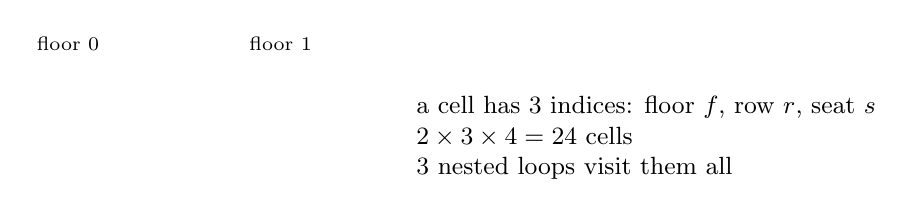
\begin{tikzpicture}
			\hGrid[id=f0, width=0.5, hot={1/2}]{{,,,},{,,,},{,,,}}
			\node[font=\scriptsize] at (1.0,0.95) {floor 0};
			\hGrid[id=f1, at={(2.7,0)}, width=0.5, hot={0/0,2/3}]{{,,,},{,,,},{,,,}}
			\node[font=\scriptsize] at (3.7,0.95) {floor 1};
			\node[font=\small, anchor=west, align=left] at (5.3,-0.25) {%
				a cell has 3 indices: floor $f$, row $r$, seat $s$\\
				$2 \times 3 \times 4 = 24$ cells\\
				3 nested loops visit them all};
		\end{tikzpicture}
	\end{center}

	\begin{itemize}\small
		\item A 3D array is a list of tables, as a table is a list of rows
		\item Examples: seats on floors, temperatures per city, week and day, the color channels of an image
		\item Every pattern works per table, per row or per cell; first choose which index stays fixed
	\end{itemize}
\end{frame}
% ~~~~~~~~~~~~~~~~~~~~~~~~~~~~~~~~~~~~~~ A frm




% ~~~~~~~~~~~~~~~~~~~~~~~~~~~~~~~~~~~~~~ V frm
\begin{frame}[t,fragile] \frametitle{N dimensions}


% +++++++++++++++++++++++++++++++++++++++ V tbl
%: -Tbl. dimensions
\begin{table}
		\small
		\begin{tabular}{@{}L{0.08\textwidth}L{0.20\textwidth}L{0.16\textwidth}L{0.20\textwidth}L{0.24\textwidth}@{}}
			\toprule
			\textbf{N} & \textbf{Picture} & \textbf{Indices} & \textbf{Cells, size 10 each} & \textbf{Example} \\
			\midrule
			1 & a list            & $i$            & 10              & scores of one student \\
			2 & a table           & $r, c$         & 100             & students $\times$ quizzes \\
			3 & a list of tables  & $f, r, c$      & 1\,000          & floors $\times$ rows $\times$ seats \\
			4 & a table of tables & four           & 10\,000         & rarely seen \\
			N & --                & N              & $10^{N}$        & grows very fast \\
			\bottomrule
		\end{tabular}
\end{table}%
% +++++++++++++++++++++++++++++++++++++++ A tbl


	\vspace{0.5em}
	\begin{itemize}\small
		\item Every new dimension adds one index and one loop, and multiplies the number of cells
		\item An N-dimensional array is a list of (N $-$ 1)-dimensional arrays
	\end{itemize}
\end{frame}
% ~~~~~~~~~~~~~~~~~~~~~~~~~~~~~~~~~~~~~~ A frm




% ~~~~~~~~~~~~~~~~~~~~~~~~~~~~~~~~~~~~~~ V
\hSection[Summary]{Summary}
% ~~~~~~~~~~~~~~~~~~~~~~~~~~~~~~~~~~~~~~ A




% ~~~~~~~~~~~~~~~~~~~~~~~~~~~~~~~~~~~~~~ V frm
\begin{frame}[t,fragile] \frametitle{Cheat sheet}


% +++++++++++++++++++++++++++++++++++++++ V tbl
%: -Tbl. cheat sheet
\begin{table}
		\small
		\begin{tabular}{@{}L{0.26\textwidth}L{0.66\textwidth}@{}}
			\toprule
			\textbf{Idea} & \textbf{In one line} \\
			\midrule
			table          & one name, cells in rows and columns, one type \\
			cell $(r, c)$   & row first, then column; both from 0 \\
			row-major      & $k = r \cdot m + c$: the order of a row-by-row visit \\
			rows           & a table is a list of references to rows \\
			ragged         & rows of different lengths; ask for the length of row $r$ \\
			shallow / deep & copy the references only / copy every row too \\
			visits         & row by row, column by column, a diagonal, the neighbors \\
			patterns       & per row, per column, every cell; keep a place $(r, c)$ \\
			N dimensions   & N indices, N loops, cells multiply \\
			\bottomrule
		\end{tabular}
\end{table}%
% +++++++++++++++++++++++++++++++++++++++ A tbl
\end{frame}
% ~~~~~~~~~~~~~~~~~~~~~~~~~~~~~~~~~~~~~~ A frm




% ~~~~~~~~~~~~~~~~~~~~~~~~~~~~~~~~~~~~~~ V frm
\begin{frame}[t,fragile] \frametitle{Exercises (paper and pencil)}
	\begin{enumerate}\small
		\item Draw a $3 \times 4$ table and number its cells in column-major order. Give the formula for $k$.
		\item Write RowAverages($t$) and ColumnMaximum($t$) as pseudo code.
		\item For a $5 \times 5$ table, which cells have exactly 3 neighbors? Exactly 2?
		\item A ragged table has rows of lengths 1, 2, 3, 4. How many cells? Which questions about it make no sense?
		\item Draw the references after a shallow copy, then after changing one cell of the copy.
		\item Transpose a $3 \times 3$ table in place: which pairs of cells are swapped, and how many?
	\end{enumerate}
\end{frame}
% ~~~~~~~~~~~~~~~~~~~~~~~~~~~~~~~~~~~~~~ A frm




% ~~~~~~~~~~~~~~~~~~~~~~~~~~~~~~~~~~~~~~ V frm
\begin{frame}[t,fragile] \frametitle{Where to go next}
	\begin{itemize}
		\item The same ideas as Java programs: \hCode{arrayND-5-examples}
		\item First steps and the common errors in Java: \hCode{arrayND-1-freshman}
		\item Library, tests and input: \hCode{arrayND-2-sophomore}
		\item Matrices, ragged structures, performance: \hCode{arrayND-3-junior}
		\item Inside the JVM, limits, security: \hCode{arrayND-4-senior}
		\item Arrays of one dimension: \hCode{array1D-0-concepts}
	\end{itemize}
\end{frame}
% ~~~~~~~~~~~~~~~~~~~~~~~~~~~~~~~~~~~~~~ A frm




% ~~~~~~~~~~~~~~~~~~~~~~~~~~~~~~~~~~~~~~ V frm
\begin{frame}[t,fragile] \frametitle{References}
	\small Arrays and orthogonal lists \cite{knuth1973artv1}; the Java Tutorials \cite{TheJavaTutorialsArray}.

	\vspace{1em}
	\setbeamertemplate{bibliography item}[text]
	\bibliographystyle{IEEEtran}
	\tiny\bibliography{../../hblib/hblibDataStructures}
\end{frame}
% ~~~~~~~~~~~~~~~~~~~~~~~~~~~~~~~~~~~~~~ A frm




% ~~~~~~~~~~~~~~~~~~~~~~~~~~~~~~~~~~~~~~ V frm
\begin{frame}[t,fragile]
	\begin{center}
		\vspace{4cm}
		\hRemark{\Huge Questions?}
	\end{center}
\end{frame}
% ~~~~~~~~~~~~~~~~~~~~~~~~~~~~~~~~~~~~~~ A frm



\end{document}
